\documentclass[11pt,letterpaper]{article}

\usepackage{graphicx}
\usepackage[margin=0.90in]{geometry}
\usepackage[T1]{fontenc}
\usepackage[utf8]{inputenc}
\usepackage{authblk}
\usepackage{fancyhdr}
\usepackage{lastpage}
\usepackage[parfill]{parskip}
\usepackage{subcaption}

\pagestyle{fancyplain}
\fancyhf{}
\fancyfoot[R]{\footnotesize Page \thepage\ of \pageref{LastPage}}

\renewcommand{\headrulewidth}{0.0pt} % No header rule
\renewcommand{\footrulewidth}{0.4pt} % Thin footer rule

\begin{document}

\title{Virtual Actor Space for On Demand Distributed Computation}
\author[1]{Benjamin Bengfort}
\author[2]{Allen Leis}
\author[1]{Konstantinos Xirogiannopoulos}
\affil[ ]{Department of Computer Science}
\affil[ ]{University of Maryland}
\affil[1]{\textit{\{bengfort,kostasx\}@cs.umd.edu}}
\affil[2]{\textit{aleis@umd.edu}}

\date{October 21, 2015}

\maketitle
\section*{Introduction}
The widespread adoption of distributed computing frameworks and tools has led to a ``data flow'' model of data analysis. Data flows are described as directed graphs whose nodes represent a single computation and whose edges represent data transmission of input and output values. Describing computation this way is simple, flexible, and when mapped to a distributed topology, scalable. Another model of computation that has been re-emerging is what is known as the ``actor model", which focuses on defining an intuitive layer of abstraction that allows users to easily reason about and deal with a lot of difficult problems in concurrent computation systems.

The traditional actor model~\cite{hewitt1973universal}, has been implemented in modern frameworks such as Akka and Erlang/lixir revolves around the idea that in order to make sense of distributed computing, we must abstract each entity into a high level primitive called an ``actor" so that everything on the system is an actor. Actors embody all essential elements of computation namely : (1) processing, (2) state, and (3) communication. In this actor world, computation happens by actors communicating with each-other through messages, processing information and altering their state.

% Why data flow model is not sufficient/ why the actor model for distributed computation would be beneficial
As described above, apart from providing an intuitive abstraction, the power of the actor model is derived from the fact that computation is not steered towards only one direction like in the ``data flow" model. The data flow model requires computation to flow from a set of computation nodes towards other ones in a single unified stream through a Directed Acyclic Graph whereas in the actor model, actors are free to exchange messages freely with eachother throughout the system with no restrictions on the direction in which the data is flowing because actors unlike data flow spouts, are stateful.


\begin{figure}[h]
	\centering
    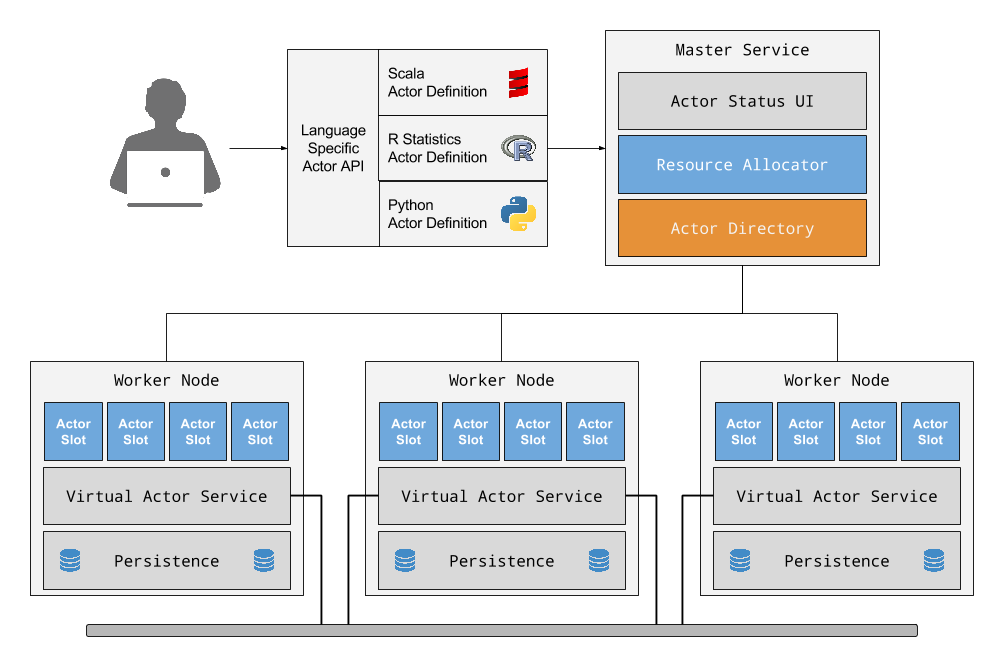
\includegraphics[width=0.8\textwidth]{figures/architecture.png}
    \caption{\textsf{Proposed architecture of a virtual actor space that generalizes distributed computation in an on demand fashion. A master node controls job submission and resource allocation, while worker nodes instantiate Actors in actor slots.}}
    \label{fig:performance}
\end{figure}

Applications that we we can implement to motivate the idea of GVAS and experiment on to show performance/benefits over other models:

\begin{enumerate}
	\item Email Analytics Dataflow using the actor model
	\item Domain decomposition (Game of Life using the actor model)
	\item Book Recommendation system
\end{enumerate}

\bibliographystyle{plain}
\bibliography{papers}

\end{document}
